\documentclass{beamer}

\usepackage[spanish]{babel}
\usepackage[utf8x]{inputenc}
\usepackage{beamerthemesplit}

\title{Instanciación Óptima de Flujos de Trabajo Abstractos Usando Lógica y Circuitos}
\author{Daniel Izquierdo}
\date{26 de marzo de 2010}

\newcommand{\qrule}{:\!\!-}
\newcommand{\vuelo}{\text{\it vuelo}}
\newcommand{\ciudadVE}{\text{\it ciudadVE}}
\newcommand{\nacional}{\text{\it nacional}}
\newcommand{\ida}{\text{\it ida}}
\newcommand{\unaescala}{\text{\it una-escala}}
\newcommand{\vueloCCS}{\text{\it vuelo-hacia-ccs}}
\newcommand{\unaparadaCCS}{\text{\it unaescala-hacia-ccs}}
\newcommand{\desdeVAL}{\text{\it desde-val}}
\newcommand{\PA}{\text{CCS}}
\newcommand{\NY}{\text{VAL}}
\newcommand{\AL}{\text{AL}}

\begin{document}

\frame{\titlepage}

%%%%%%%%%%%%%%%%%%%%%%%%%%%%%%%%%%%%%%%%%%%%%%%%%%%%%%%%%%%%%%%%%%%%%%%%%%%%%%%%

\section[Contenido]{}
\frame{\tableofcontents}

%%%%%%%%%%%%%%%%%%%%%%%%%%%%%%%%%%%%%%%%%%%%%%%%%%%%%%%%%%%%%%%%%%%%%%%%%%%%%%%%

\section{Motivación}
\frame
{

\begin{itemize}
\item Explosión en número de servicios y fuentes de datos disponibles
\item Heterogeneidad de servicios concretos y fuentes
\item Diferencias en calidad de servicio existentes en el mundo real
    \item Necesidad de realizar consultas o \emph{workflows} bajo estas condiciones
\end{itemize}
}

%%%%%%%%%%%%%%%%%%%%%%%%%%%%%%%%%%%%%%%%%%%%%%%%%%%%%%%%%%%%%%%%%%%%%%%%%%%%%%%%

\section{Objetivo}
\frame
{
Desarrollar un sistema eficiente y escalable que pueda resolver problemas de
reescritura de consultas o composición de servicios con constantes, tomando en
cuenta parámetros de calidad para obtener una mejor solución.
}

%%%%%%%%%%%%%%%%%%%%%%%%%%%%%%%%%%%%%%%%%%%%%%%%%%%%%%%%%%%%%%%%%%%%%%%%%%%%%%%%

\section{Ejemplo}

\subsection{Servicios abstractos y consulta}

\frame
{
    \begin{itemize}
    \item Servicios abstractos:
        \begin{itemize}
        \item $\vuelo(x,y)$
        \item $\ciudadVE(x)$
        \end{itemize}
    \item Consulta:\\ $W(x,w,y,z) \qrule$\\ $\ciudadVE(x),\,\vuelo(x,w),\,\vuelo(w,y),\,\vuelo(y,z),\,\vuelo(z,x)$
    \end{itemize}
}

\subsection{Servicios concretos}

\frame
{
\begin{itemize}
\item {\tiny $\nacional(x,y)$ relaciona dos ciudades de Venezuela conectadas por un vuelo directo,} \\
      {\tiny $\nacional(x,y)\   \qrule\ \vuelo(x,y),\,\ciudadVE(x),\,\ciudadVE(y)$}\\
\item {\tiny $\ida(x,y)$ relaciona dos ciudades conectadas por un vuelo de ida,}\\
      {\tiny $\ida(x,y)\     \qrule\ \vuelo(x,y)$}\\
\item {\tiny $\unaescala(x,y)$ relaciona dos ciudades conectadas por un vuelo con una escala,}\\
      {\tiny $\unaescala(x,z)\    \qrule\ \vuelo(x,y),\,\vuelo(y,z)$}\\
\item {\tiny $\vueloCCS(x)$ dice si hay un vuelo directo desde $x$ a Caracas,}\\
      {\tiny $\vueloCCS(x)\     \qrule\ \vuelo(x,\PA)$}\\
\item {\tiny $\unaparadaCCS(x,y)$ relaciona $x$ y $y$ si hay un vuelo desde $x$ a Caracas con una escala en $y$,}\\
      {\tiny $\unaparadaCCS(x,y)\  \qrule\ \vuelo(x,y),\,\vuelo(y,\PA)$}\\
\item {\tiny $\desdeVAL(x)$ dice si hay un vuelo de Valencia a $x$,}\\
      {\tiny $\desdeVAL(x)\       \qrule\ \vuelo(\NY,x)$}\\
\end{itemize}
}

\subsection{Composiciones}

\frame
{
    Pueden existir composiciones válidas
{\tiny $$I(x,w,y,z)\ \qrule\ \nacional(x,w),\,\vueloCCS(w),\,\ida(\PA,z),\,\nacional(z,x)$$}

    y no válidas

{\tiny $$I'(x,w,y,z)\  \qrule\ \nacional(x,y),\,\vueloCCS(y),\,\desdeVAL(z),\,\nacional(z,x)$$\\
       $$I''(x,w,y,z)\ \qrule\ \unaescala(x,y),\,\ida(y,z),\,\nacional(z,x)$$\\
}
}

%%%%%%%%%%%%%%%%%%%%%%%%%%%%%%%%%%%%%%%%%%%%%%%%%%%%%%%%%%%%%%%%%%%%%%%%%%%%%%%%

\section{Retos}
\frame
{
\begin{itemize}
\item Gran número de fuentes o servicios.
\item Manejo de transitividad en asociaciones de variables con constantes.
\end{itemize}
}

%%%%%%%%%%%%%%%%%%%%%%%%%%%%%%%%%%%%%%%%%%%%%%%%%%%%%%%%%%%%%%%%%%%%%%%%%%%%%%%%

\section{Solución Propuesta}
\frame
{
\begin{enumerate}
\item Traducir instancias del problema a instancias de SAT (ya realizado).
\item Añadir cláusulas para tratar con constantes.
\item Compilar teorías a d-DNNF.
\item Calcular todas las reescrituras -- o la mejor.
\end{enumerate}
}

%%%%%%%%%%%%%%%%%%%%%%%%%%%%%%%%%%%%%%%%%%%%%%%%%%%%%%%%%%%%%%%%%%%%%%%%%%%%%%%%

\section{Estudio Experimental}

\subsection{Vuelos con escalas y aerolíneas}
\frame
{
    Primer experimento: búsqueda de vuelos con $n$ escalas usando la misma
    aerolínea para todas las escalas.
}

\frame
{

\begin{center}
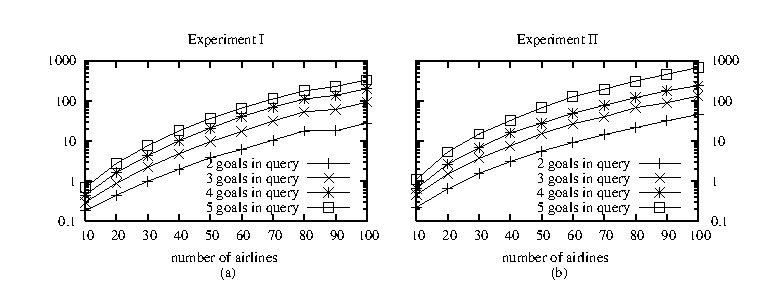
\includegraphics[width=0.5\textwidth]{plot1}
\end{center}

\begin{itemize}
\item Instancias de tamaños realistas
\item Buenos tiempos incluso para las instancias más grandes
\end{itemize}

Esto incluye cálculo de todas las reescrituras o de la mejor.
}

\subsection{Otros experimentos}
\frame
{
\begin{itemize}
\item Con dos vistas por aerolínea: compilación un minuto en caso más grande
\item Menos de seis minutos para problema aleatorio con
\begin{itemize}
\item 80 vistas
\item 5 objetivos de consulta
\item 4 predicados por vista
\end{itemize}

\end{itemize}

Tiempos dados para cálculo de todas las reescrituras.
}

%%%%%%%%%%%%%%%%%%%%%%%%%%%%%%%%%%%%%%%%%%%%%%%%%%%%%%%%%%%%%%%%%%%%%%%%%%%%%%%%

\section{Conclusiones y Trabajo Futuro}

\frame
{
\begin{itemize}
\item Se puede escalar a tamaños razonables.
\item Es factible manejar constantes y rendimiento con la aproximación
propuesta.
\item Queremos aun más escalabilidad: posible combinación de este
sistema con algoritmo tipo branch and bound, o Max-Sat solvers.
\end{itemize}
}

\end{document}
